%!TEX root = main.tex


%\gnote{Write the paper in the client-server model, where the client can hold $4$ buckets at a time; Write the introduction as such; Move all other optimizations to "extensions"}

\section{Introduction}

With the increased use of outsourced storage and computation, privacy of the outsourced data has been of paramount importance. 
A canonical setting is where a client with a small local
storage outsources its encrypted data to an untrusted server. 
In this setting, encryption alone is not sufficient to preserve privacy.
The access patterns to the data may reveal sensitive information. 

Two fundamental building blocks for oblivious storage and computation~\cite{goldreich1996software,goodrich2011privacy,oblivistore} are oblivious sorting and oblivious random permutation.
In these two problems, an array of $n$ elements is stored on an untrusted server, encrypted under a trusted client's secret key.
The client wishes to sort or permute the $n$ elements in a \emph{data-oblivious} fashion.
That is, the sequence of accesses it makes to the server should not reveal any information about the $n$ elements (e.g., their relative ranking).
The client has a small amount of local storage, the access pattern to which cannot be observed by the server.
This work presents simple and efficient algorithms to these problems, named bucket oblivious sort and bucket oblivious random permutation.

\subsection{State of the Affairs.}
For oblivious sort, it is well-known that one can leverage 
sorting networks such as AKS~\cite{aks} and Zig-zag sort~\cite{zigzag}
to obliviously sort $n$ elements in $O(n\log n)$ time. 
Unfortunately, these algorithms are complicated and incur enormous constants rendering them completely impractical. 
%\rl{What's expensive is approximate halvers, not expanders.} 
Thus, almost all known practical implementations~\cite{oblivistore,oblivm,graphsc}
instead employ the simple bitonic sort algorithm~\cite{bitonic}. 
While asymptotically worse, due to the small leading constants, it performs much better in practice.

Oblivious random permutation (ORP) can be realized by assigning a sufficiently long random key to each element, and then obliviously sorting the elements by the keys.
To the best of our knowledge, this remains the most practical solution for ORP.
It then follows that while $O(n \log n)$ algorithms exist in theory, practical instantiations resort to the $O(n \log^2 n)$ bitonic sort.
There exist algorithms such as the Melbourne
shuffle~\cite{ohrimenko2014melbourne} that do not rely on
oblivious sort; but they require $O(\sqrt{n})$ client storage to permute $n$ elements.
Other approaches include the famous Thorp shuffle~\cite{thorp01} and random permutation networks~\cite{randpermnet}, but none of these solutions are competitive in performance either asymptotically or concretely.

\subsection{Our Results.}
Let $Z$ be a statistical security parameter that controls the error probability. 
Our bucket oblivious sort runs in $6n\log n$ time ($4n\log n$ for bucket ORP) and has an error probability around $e^{-Z/6}$ when the client can store $2Z$ elements locally.
This is at most $3\times$ slower than the non-oblivious merge sort, and is at least $5\times$ faster than bitonic sort for $n=2^{30}$ (cf. Table~\ref{tab:compare}).
Therefore, we recommend bucket oblivious sort and ORP as attractive alternatives to bitonic sort in practical implementations.

\begin{figure*}[h!]
\centering
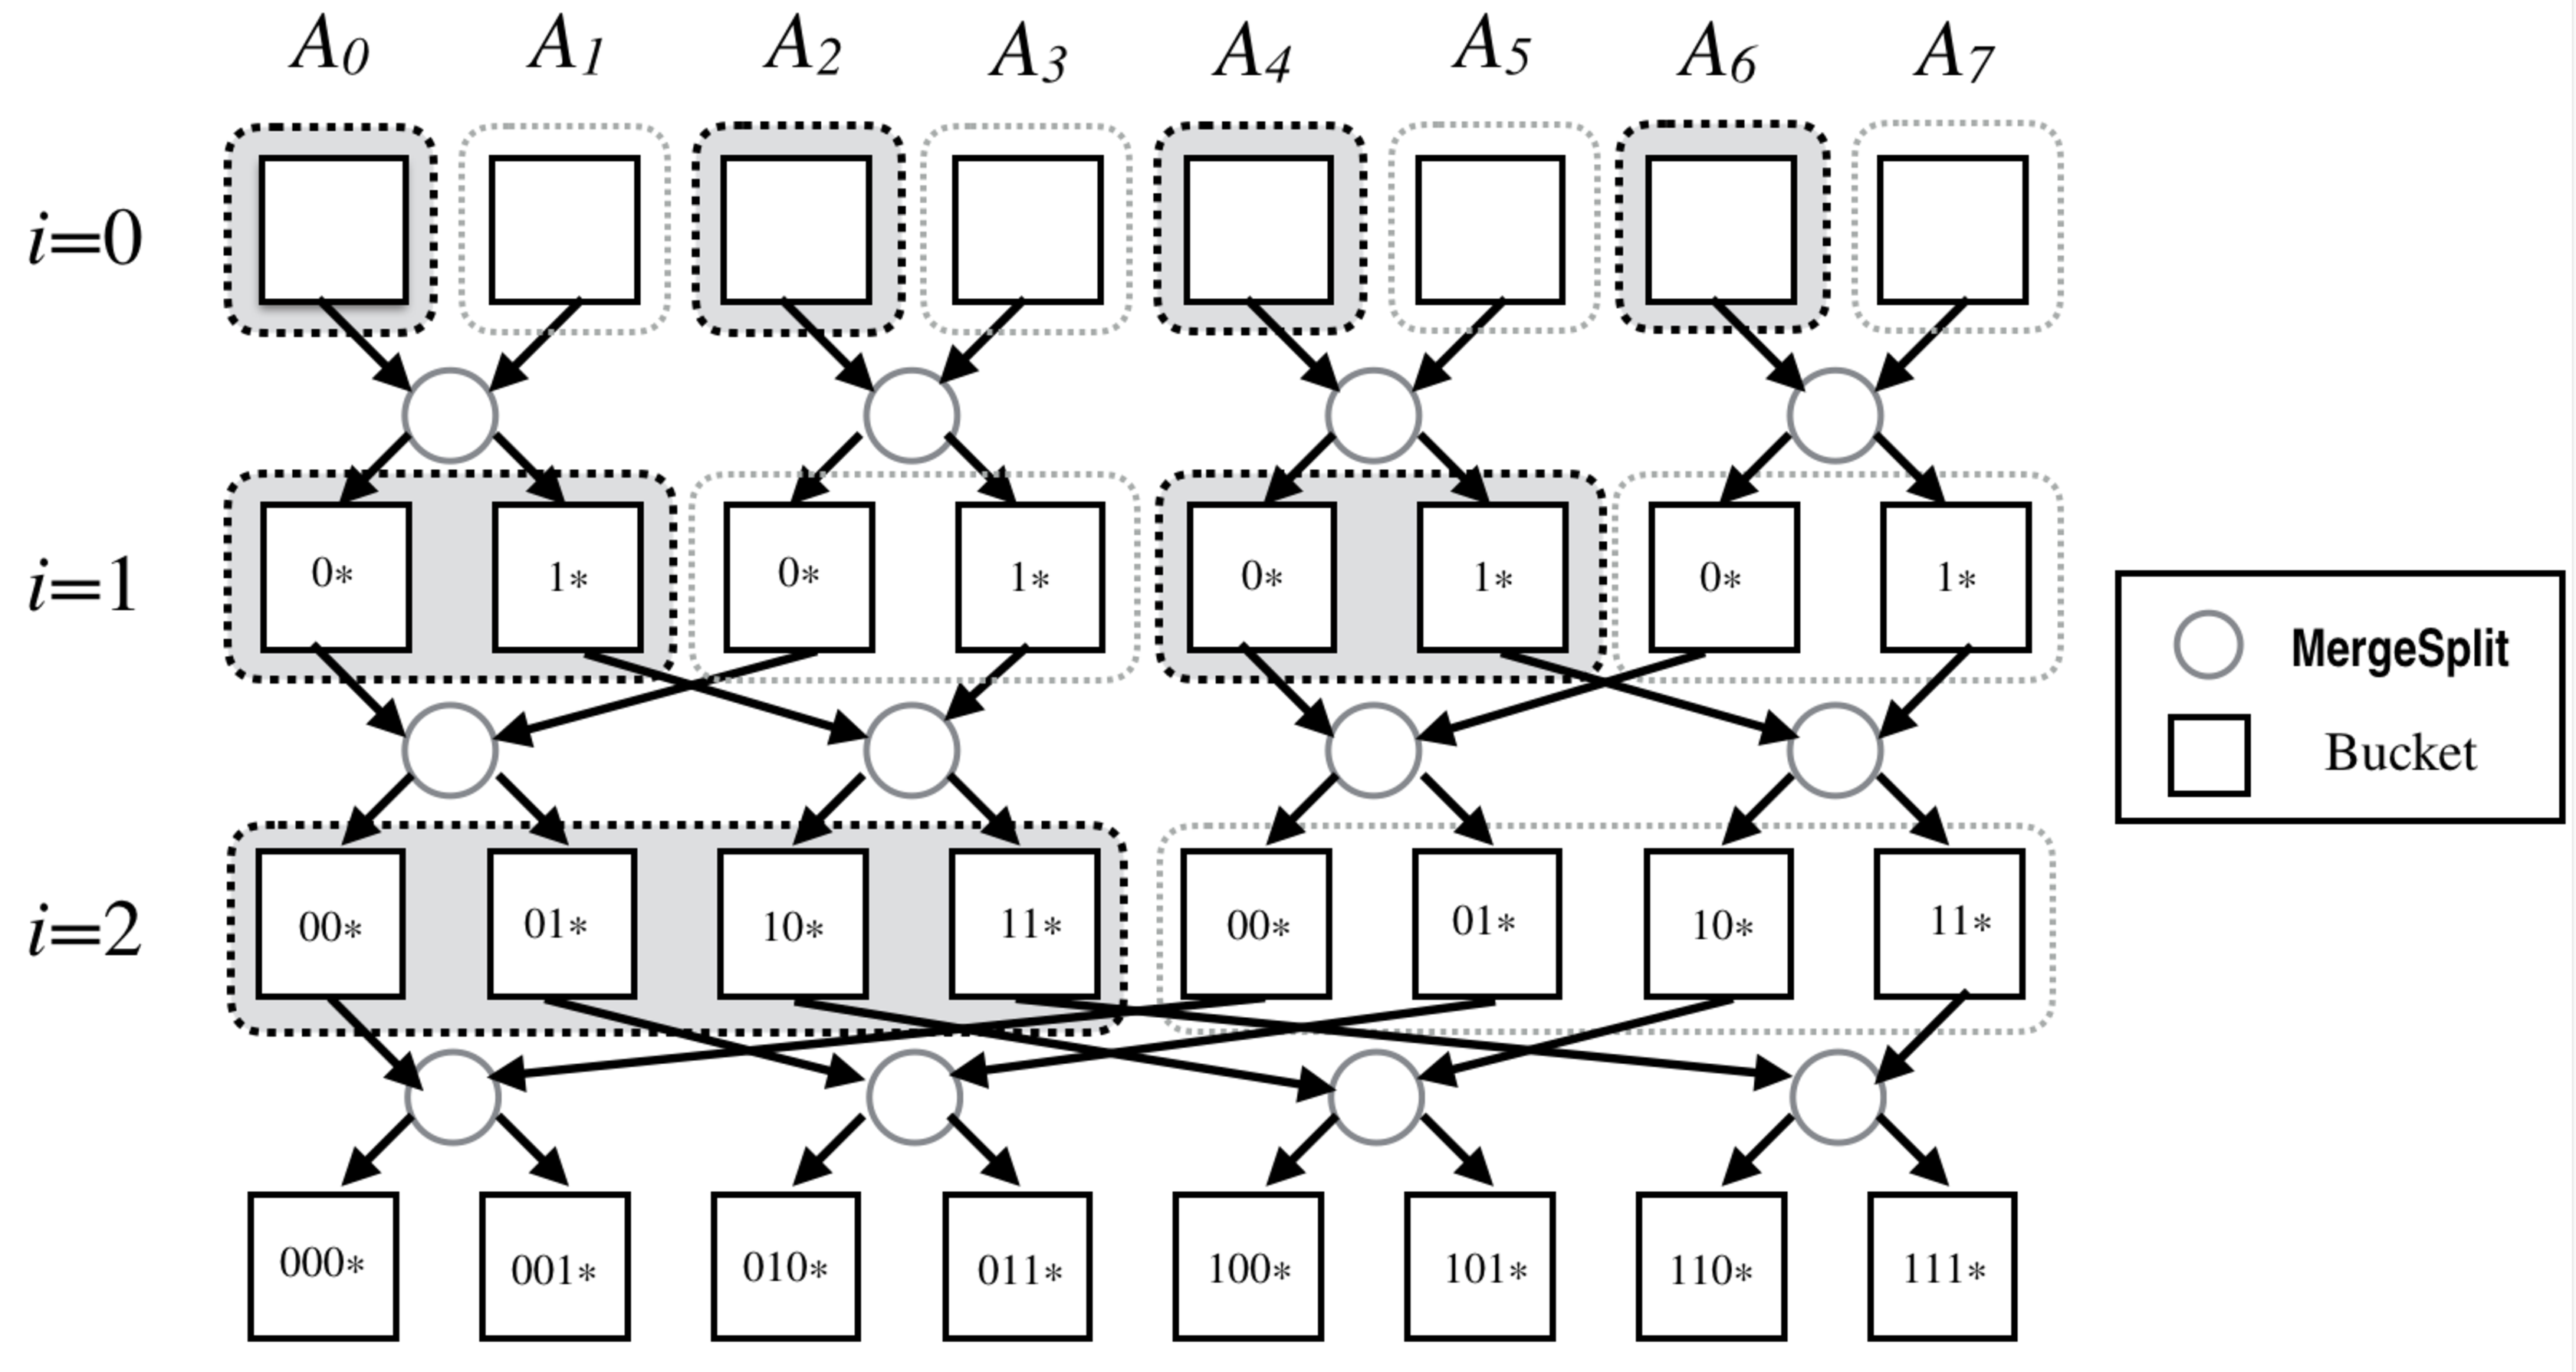
\includegraphics[width=0.7\textwidth]{RadixBucketSort1.pdf}
\captionof{figure}{\textbf{Oblivious random bin assignment with 8 buckets.}
The \textsc{MergeSplit} procedure takes elements from two buckets at level $i$ and put them into two buckets at level $i+1$, according to the $(i+1)$-th most significant bit of the keys. 
At level $i$, every $2^{i}$ consecutive buckets are semi-sorted by the most significant $i$ bits of the keys.}
\label{fig:radix-sort}

%\begin{table*}[t]
\bigskip
\centering
\begin{tabular}{|c|c|c|c|c|}
    \hline
    Algorithm & Oblivious & Client storage & Runtime & Error probability \\
    \hline
    Merge sort & No & $O(1)$ & $2n \log n$ & 0 \\
    Bitonic sort & Yes & $O(1)$ & $n\log^2 n$ & 0 \\
    AKS sort~\cite{aks} & Yes & $O(1)$ & $5.4\times10^7 \times n\log n$ & 0 \\
    Zig-zag sort~\cite{zigzag} & Yes & $O(1)$ & $8\times10^4 \times n\log n$ & 0 \\
    Randomized Shellsort~\cite{RandShellsort} & Yes & $O(1)$ & $24n\log n$ & $\approx n^{-3}$ \\
    \hline
    \textbf{Bucket oblivious sort} & Yes & $2Z$ & $6 n\log n$ & $\approx e^{-Z/6}$\\
    \textbf{Bucket oblivious sort} & Yes & $O(1)$ & $\approx 2n\log n \log^2 Z$ & $\approx e^{-Z/6}$ \\
    \hline   
\end{tabular}
\captionof{table}{\textbf{Runtime of bucket oblivious sort and
classic non-oblivious and oblivious sort algorithms.} Bitonic
sort requires $\frac 14 n \log^2 n$ comparisons. The number of comparisons for AKS
sort and zig-zag sort are cited from \cite{zigzag}. Runtime
represents the number of memory accesses, which is four times the
number of comparisons.}
\label{tab:compare}
%\end{table*}

\end{figure*}

The core of our algorithms is to assign each element to a random bin and then route the elements through a butterfly network to their assigned random bins. 
This part is inspired by Bucket ORAM~\cite{fletcher2015bucket}. 
In more detail, we divide the $n$ elements into $B=2n/Z$ buckets of size $Z/2$ each and add $Z/2$ dummy elements to each bucket.
Now, imagine that these $B$ buckets form the inputs of a butterfly network --- for simplicity, assume $B$ is a power of two.
Each element is uniformly randomly assigned to one of the $B$ output buckets, represented by a key of $\log B$ bits.
The elements are then routed through the butterfly network to their respective destinations.
Assuming the client can store two buckets locally at a time, at level $i$, the client simply reads elements from two buckets that are distance $2^i$ away in level $i$ and writes them to two adjacent buckets in level $i+1$, using the $i$-th bit of each element's key to make the routing decision. 
We refer readers to Figure~\ref{fig:radix-sort} for a graphical illustration.

The above algorithm is clearly oblivious, as the order in which the client reads and writes the buckets is fixed and independent of the input array. If no bucket overflows, all elements reach their assigned destinations. By setting $Z$ appropriately, we can bound the overflow probability.

Our bucket oblivious sort and bucket ORP algorithms are derived from
this oblivious random bin assignment building block. 

\paragraph{From oblivious bin assignment to ORP and oblivious sort.}
To obtain a random permutation, we simply remove all dummy elements and randomly permute 
each bucket of the final layer.
Since the client can hold $Z$ elements, permuting each bucket can be done locally. 
We show that the algorithm is oblivious and gives a random permutation despite revealing the number of dummy elements in each destination bucket.
To get oblivious sort, we can first perform ORP on the input array then apply any \emph{non-oblivious, comparison-based} sorting algorithm (e.g., quick sort or
merge sort). We show that the composition of ORP and non-oblivious sort results in an oblivious sort. 

\paragraph{Dealing with small client storage.}
In Section~\ref{sec:O1client}, we extend the above algorithm
to support $O(1)$ client storage. 
We can rely on bitonic sort to realize the \textsc{MergeSplit} operation that operates on 4 buckets at a time,
which would result in $O(n\log n\cdot \log^2 Z)$ runtime. 

\paragraph{Locality.} Algorithmic performance when the data is stored on disk has been studied in the external disk model (e.g.,~\cite{RuemmlerW94,ArgeFGV97,Vitter01,Vitter06}) and references within). Recently, Asharov et al.~\cite{AsharovCNPRS19} extended this study to oblivious algorithms.  We observe that our algorithm is locality-friendly, and refer the reader to Section~\ref{sec:locality} for the exact definitions and the complexity measure.


%\paragraph{Organization.}
%The rest of the paper is organized as follows. Our algorithms are simple and intuitive. The access pattern of all our algorithms is deterministic, and therefore security is trivial and all we have to prove is correctness. In Section~\ref{sec:construction} we give our construction and in Section~\ref{sec:extensions} we describe simple extensions. In Appendix~\ref{sec:defs}  define the RAM model of computation and obliviousness. In Appendix~\ref{appx:formal} we give all omitted proofs. 

%
%
%\paragraph{From oblivious bin assignment to ORP.}
%To obtain a random permutation, a simple approach is to remove the dummy elements and permute within each bucket of the final layer. Since the client can hold $Z$ elements, permuting each bucket obliviously can be done locally. 
%
%
%Our bucket oblivious sort and bucket ORP build on top of the above oblivious random bin assignment. 
%To get ORP, simply remove all dummy elements, randomly permute each bucket of the final level, and concatenate the bins.
%To sort, we can simply apply any non-oblivious comparison-based sort (e.g., merge sort) on the randomly permuted elements. 
%
%In Section~\ref{sec:O1client}, we will discuss how to extend our algorithms to support constant client storage
%We can rely on Bitonic sort to realize the ${\bf MergeSplit}$ operation, which would result in $\approx 2n\log n \log^2 Z$ runtime.
%Recently, Asharov et al.~\cite{AsharovCNPRS19} initiate the study of data locality on oblivious algorithms. 
%We observe that our algorithms are be made locality-friendly, and refer readers to Appendix~\ref{sec:locality} for the exact definitions and complexity measures.

%%% Local Variables:
%%% mode: latex
%%% TeX-master: "main"
%%% End:
